\chapter{Result Analysis}
After building all of our algorithms and drawing figures, we showed all the related results here with a prediction result in this segment.\\

We use pandas and yfinance to extract the DJIA value from Yahoo Finance.The yfinance module is a Python module that is very simple to use. The module 'yfinance' has grown in popularity as a python-friendly library that can be used as a patch to pandas datareader or as standalone library.  It has a wide range of applications, and many people use it to download stock and cryptocurrency prices. Let's pretend we want to work with Google Finance's Close prices, which have already been updated to account for stock splits. We want to make sure that our dataset includes all weekdays, which is important for quantitative trading techniques. As a result, we get a graph drawn in figure 4.1 which providing DJIA value stock prices average.\\
\begin{figure}[H]
    \centering
    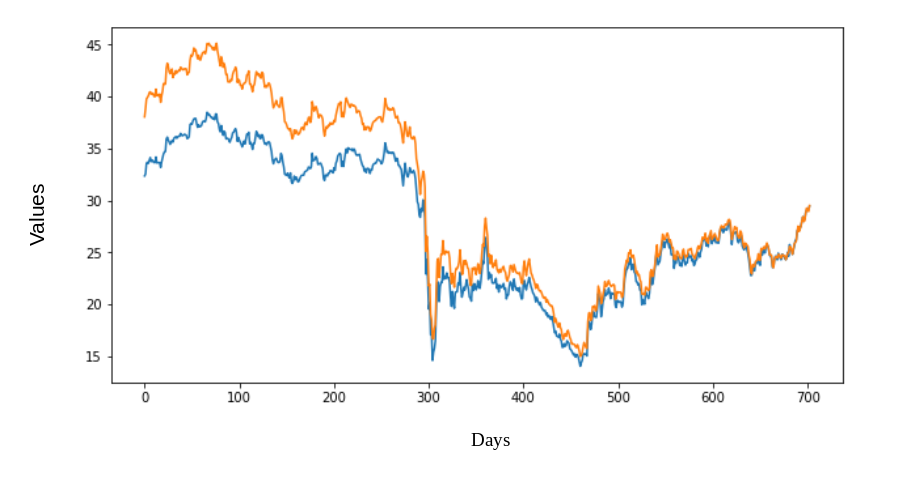
\includegraphics[scale=.5]{img4/DJIA Average.png}
    \caption{DJIA Values Stock Price Average}
    \label{fig:DJIA Average}
\end{figure}

After getting DJIA values we collected our twitter data by using our twitter data extract and collect algorithm mentioned and explained in our system model. We extracted twitter data from 2019 till now and we added here some of our twitter data extracted in 2021 that is illustrated in figure 4.2.\\
\begin{figure}[H]
    \centering
    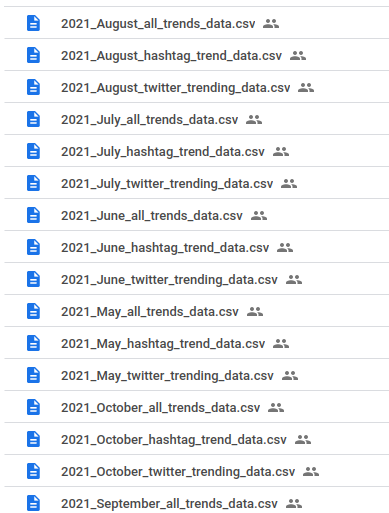
\includegraphics[scale=.8]{img4/extracttweet.png}
    \caption{Some Extracted Tweet}
    \label{fig:extracttweet}
\end{figure}

Then, we cleaned and filtered our extracted twitter data and stored in our drive for keeping it updated. We used twitter filtering algorithm and removed all types of punctuations, hashtags, emojis, tags which can be harmful to store raw data. These cleaned data will help to gain our fifth objective as every tweet is not important specially those tweets where special characters are added. We can see some of our sample cleaned tweets at the following figure 4.3 as shown below:\\
\begin{figure}[H]
    \centering
    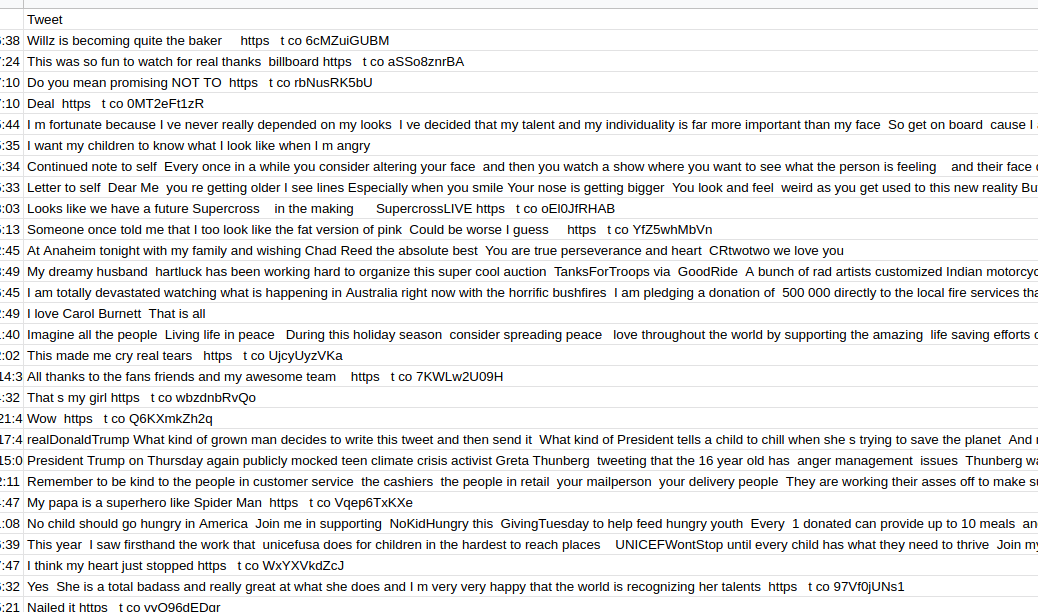
\includegraphics[scale=.5]{img4/clean.png}
    \caption{Sample Cleaned Tweets}
    \label{fig:clean}
\end{figure}

With another machine learning and neural network approach like multiple regression, SVM, and others, our result will be able to provide the closest accuracy. We attempted to develop it for better output because Linear Regression is an old conventional model.
The third objective of our work to predict by applying a proper algorithm text blob for sentiment. For the sentiment analyzer, we use textblob. After cleaning and filtering (removing hashtags, emoji, punctuation marks, and other obtrusive elements), we determine positive and negative scores from a collection of Twitter postings. Then use sentiment classification to assess subjectivity and polarity, two attributes. The float polarity which is in the range [-1,1], with 1 denoting a positive statement and -1 denoting a negative statement. Subjectivity statements which usually refer to personal feelings, emotions, or judgments, whereas objective sentences refer to facts. These graphs shown in figure 4.4 are offered to help us achieve our third goal of finding the best outcome.\\
\begin{figure}[H]
    \centering
    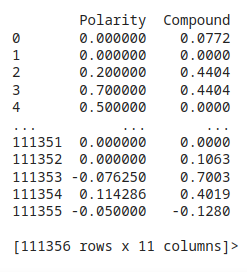
\includegraphics[scale=.9]{img4/subpol.png}
    \caption{Subjectivity and Polarity}
    \label{fig:subpol}
\end{figure}

On condition that our two number hypothesis, we have worked here with cleaned tweets and we have applied sentiment analyzer for getting positive, negative and neutral mood for a user. By analyzing or comparing we were able to show the effect of positive and negative moods specially on figure 4.5. From these values, we can determine any types of moods such as neutral, compound besides positive and negative moods of any users easily to prove our number one hypothesis.\\
\begin{figure}[H]
    \centering
    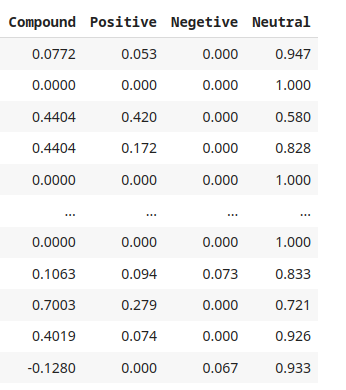
\includegraphics[scale=.9]{img4/analyzer.png}
    \caption{Sentiment Analyzer values}
    \label{fig:analyzer}
\end{figure}

To prove our first hypothesis, we have also shown a figure 4.6 which represents graph of our tweets on which we did our sentiment analyzing and tried to show it with different color for better understanding.\\
\begin{figure}[H]
    \centering
    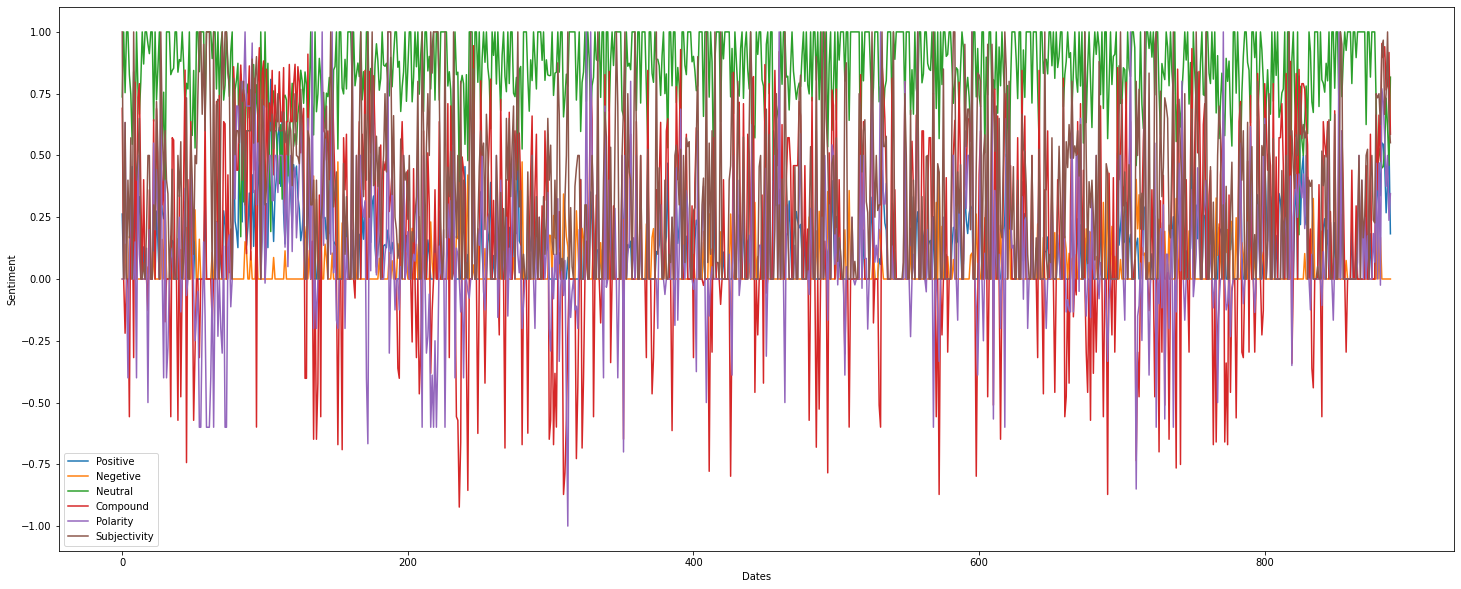
\includegraphics[scale=.3]{img4/sentiment.png}
    \caption{Sentiments of tweets}
    \label{fig:Sentiments of tweets}
\end{figure}



We have worked on our data that we acquired by applying the techniques indicated above to gain an analysis on our project. After filtering and cleaning the raw data and deleting all forms of hashtags and punctuations, we ran our linear regression, which predicted whether the price of a share would rise or fall the next day with 73 percent accuracy. From the following figure 4.7 we can display our classification report of our model and this is highly used to show the precision, recall, f1-score and support on our trained data. This classification report is used to measure the performance evaluation in any machine learning model correctly. We also tried to show the mean absolute error so that we can be able to identify or measure how much our accuracy level is better. It fulfills our second objective that means it is reducing complexity more than before and also giving higher accuracy approximately 73\% which is already mentioned. Also, this prediction helped us to prove our second hypothesis clearly.
\begin{figure}[H]
    \centering
    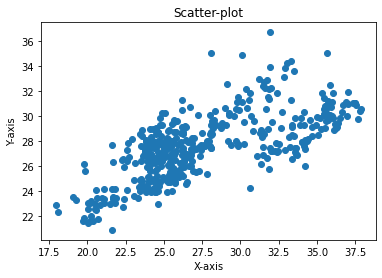
\includegraphics[scale=.6]{img4/score2.png}
    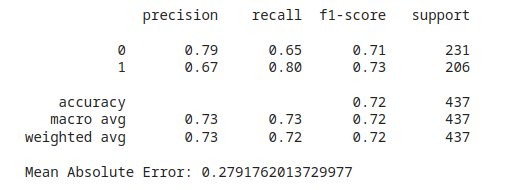
\includegraphics[scale=1]{img4/score1.png}
    \caption{Predicted Percentage}
    \label{fig:Predict}
\end{figure}
The scatter plot as shown in the figure 4.7 represents the prediction values vs real values plot where we can show the difference. Also, from the below figure we can see clearly the difference between the actual and predicted values.\\
\begin{figure}[H]
    \centering
    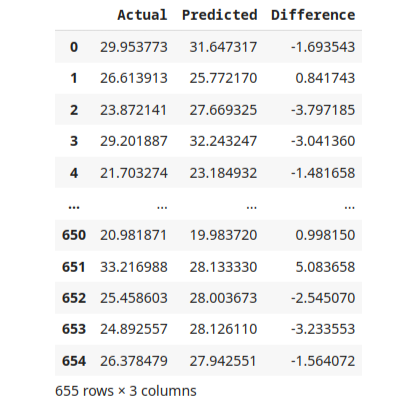
\includegraphics[scale=.6]{img4/result.png}
    \caption{Actual vs Predicted}
    \label{fig:result}
\end{figure}
From the above figure 4.8 we can see that the difference between actual and predicted value is almost close. There is no huge difference between them as we can see. Also, we showed this difference in a graph with a green and red color where actual values are seemed to green and predicted values are shown as a red color. Thorough this figure 4.9 which illustrates a graph, any one can be able to see the difference between them.\\
\begin{figure}[H]
    \centering
    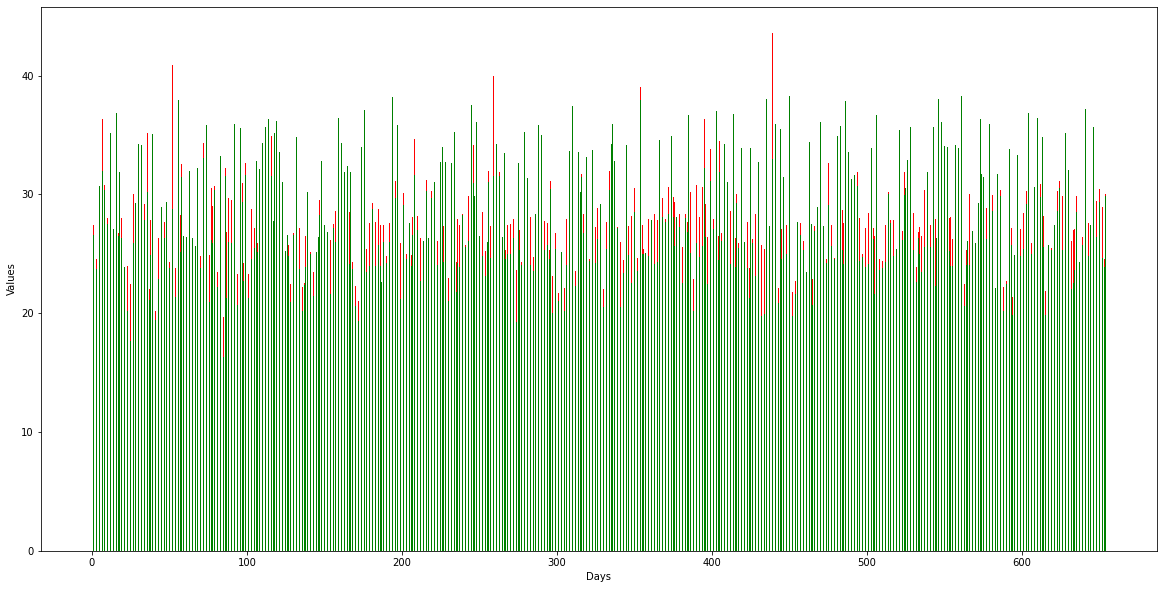
\includegraphics[scale=.35]{img4/Values.png}
    \caption{Actual values vs Predicted Values}
    \label{fig:Actual values vs Predicted Graph}
\end{figure}
Any user will be able to decide whether or not to acquire the stock, and this will be achievable if there are good sentiments; however, if the mood remains negative, the stock may need to be sold. 
With another machine learning and neural network approach like multiple regression, SVM, and others, our result will be able to provide the closest accuracy. We attempted to develop it for better output because Linear Regression is an old conventional model.\\

\section{Comparison with Other Works}
In this segment, we compare our result with other projects at the following table so that we can show where we have been able to improve. From the research gap section, we compared their accuracy, approach in detail and also discussed their drawbacks in which they can improve their projects and also added our gap which can be developed in future.\\

\begin{tabular}{ |p{2cm}|p{4cm}|p{4cm}|p{4cm}| } 
 \hline Tittle of Works
&Prediction of stock values using sentiment analysis on
twitter data \cite{prasadinternational}
&Examining the effects of pan-demics on stock market trends through sentiment analysis\cite{biswas2020examining}
&Tittle of our work "Stock Market Analysis Using Twitter Sentiment"\\ 
 \hline
 Approach 
 &The model that processes live tweets and categorizes them as good, negative, or neutral, based on Twitter data
 &A variety of news stories with numerical values in order to better comprehend stock market trends based on previous patterns 
 &Trending Tweets analyse with textblob  and sentiment analyzer for sentiment analysis  \\ 
 \hline
 Results 
 &67\% directional accuracy for DJIA
 &50\% accuracy of positive and negative value 
 &73\% accuracy for DJIA of positive, negative, compound, neutral mood \\ 
 \hline
 Feedback/ Drawbacks 
 &The results would be less accurate, hinting that the emotion of the people they analyzed isn't totally accurate. 
 &The use of aggregated share prices and the lack of daily news and articles gathered from different financial and stock market websites 
 &The proposed data-set does not represent true public mood; it only takes into account persons who use Twitter and speak English., it is feasible to establish a higher correlation.  \\ 
 \hline
\end{tabular}\\